% ============================================================================
% Lecture 17 (B16): Sequence-Space DEQNs
% Deep Learning for Solving and Estimating Dynamic Models in Economics and Finance
% Course author: Simon Scheidegger
% ============================================================================

\documentclass[aspectratio=169,11pt]{beamer}

% ---------- Theme and colors ----------
\usecolortheme{dove}
\setbeamertemplate{navigation symbols}{}
\setbeamertemplate{footline}{%
  \hfill\usebeamerfont{page number in head/foot}%
  \usebeamercolor[fg]{normal text}%
  \insertframenumber\,/\,\inserttotalframenumber\kern1em\vskip4pt}
\setbeamerfont{frametitle}{size=\huge}

% ---------- Packages ----------
\usepackage[utf8]{inputenc}
\usepackage[T1]{fontenc}
\usepackage{lmodern}
\usepackage{amsmath,amssymb,amsfonts}
\usepackage{bm}
\usepackage{graphicx}
\usepackage{tikz}
\usetikzlibrary{shapes,arrows.meta,positioning,calc,fit,backgrounds,patterns,decorations.pathreplacing}
\usepackage{pgfplots}
\pgfplotsset{compat=1.18}
\usepackage{booktabs}
\usepackage{hyperref}
\usepackage{xcolor}

% ---------- Custom colors ----------
\definecolor{uzhblue}{rgb}{0,0,0.5}
\definecolor{uzhgreylight}{RGB}{236,238,241}
\definecolor{uzhgreydark}{RGB}{81,86,94}
\definecolor{harvardcrimson}{RGB}{153,0,0}
\definecolor{unil@blue}{RGB}{0,140,204}
\definecolor{unil@black}{RGB}{35,31,32}
\definecolor{darkgreen}{RGB}{0,100,0}
\definecolor{darkred}{RGB}{139,0,0}
\definecolor{softblue}{RGB}{70,130,180}
\definecolor{softorange}{RGB}{230,159,0}
\definecolor{softgreen}{RGB}{0,158,115}

% ---------- Set beamer colors ----------
\setbeamercolor{frametitle}{bg=uzhgreylight, fg=uzhblue}
\setbeamercolor{title}{fg=uzhblue}
\setbeamercolor{structure}{fg=uzhblue}
\setbeamercolor{block title}{bg=unil@blue, fg=white}
\setbeamercolor{block body}{bg=uzhgreylight}
\setbeamercolor{block title alerted}{bg=darkred,fg=white}
\setbeamercolor{block body alerted}{bg=red!5}
\setbeamercolor{block title example}{bg=darkgreen,fg=white}
\setbeamercolor{block body example}{bg=green!5}
\setbeamercolor{item}{fg=unil@black}
\setbeamercolor{normal text}{fg=unil@black}

% ---------- Emphasis and hyperlinks ----------
\newcommand{\emphc}[1]{\textcolor{harvardcrimson}{#1}}
\hypersetup{colorlinks,linkcolor=harvardcrimson,urlcolor=harvardcrimson}

% ---------- Math commands ----------
\newcommand{\X}{\bm{X}}
\newcommand{\E}{\mathcal{E}}

% ---------- Title ----------
\title[Lecture 17 (B16)]{Lecture 17 (B16): Sequence-Space DEQNs}
\subtitle{Sequence-Space DEQNs}
\author{Simon Scheidegger}
\institute{HEC, University of Lausanne}
\date{}

\begin{document}

% =====================================================================
% Title
% =====================================================================
{\setbeamercolor{background canvas}{bg=uzhgreylight}
\begin{frame}
\titlepage
\vspace{-0.4cm}
\begin{center}
{\footnotesize Companion deck to \texttt{08\_Heterogeneous\_Agents\_Youngs\_Method}.}\\[4pt]
{\footnotesize Based on: Azinovic-Yang \& \v{Z}emli\v{c}ka (2025), Boppart et al.\ (2018), Auclert et al.\ (2021).}
\end{center}
\end{frame}
}

% =====================================================================
% PART I -- MOTIVATION
% =====================================================================

\begin{frame}{Motivation}
\small
\begin{itemize}\itemsep6pt
\item Globally solving models with rich \emphc{heterogeneity} and \emphc{aggregate risk} is hard.
    \begin{itemize}
        \item[$\rightarrow$] high-dimensional \emphc{endogenous} aggregate state (a distribution $\mu_t$).
    \end{itemize}

\item \emphc{Sequence-space idea:} approximate equilibrium objects as a function of a \emphc{truncated history of aggregate shocks}.
\[
\underbrace{\mathcal{V}\bigl(a_t,\, z_t,\, \mu_t,\, \varepsilon_t\bigr)}_{\text{state-space form}}
\;=\;
\underbrace{\mathcal{V}\bigl(a_t,\, z_t,\, \{\varepsilon_i\}_{i=0}^{t}\bigr)}_{\text{sequence-space form}}
\;\approx\;
\underbrace{\mathcal{V}\bigl(a_t,\, z_t,\, \{\varepsilon_i\}_{i=t-\tau}^{t}\bigr)}_{\text{truncated sequence form}}
\]

\item Truncated history is high-dimensional, but \emphc{exogenous}.
\item Can deep learning approximate equilibrium objects on this exogenous domain?
\end{itemize}
\end{frame}


\begin{frame}{What this lecture covers}
\small
\begin{block}{Today: the Brock--Mirman warm-up}
The simplest setting in which the history-to-policy idea is visible. One representative household, one aggregate shock, an analytic policy under $\delta=1$, log utility for cross-checking.
\end{block}

\begin{block}{Two paper-level ingredients (Azinovic-Yang \& \v{Z}emli\v{c}ka, 2025)}
\begin{enumerate}\itemsep1pt
    \item Approximate equilibrium objects as a function of \emphc{truncated histories} -- exogenous domain. \;\textbf{(covered today)}
    \item Parameterise via \emphc{shape-preserving neural networks} -- monotonicity / concavity guarantees. \;\textbf{(pointer only)}
\end{enumerate}
\end{block}

\begin{block}{In-class notebooks (this morning)}
\texttt{05\_SequenceSpace\_BrockMirman.ipynb} -- the warm-up that isolates the history-to-policy logic.\\
\texttt{05b\_SequenceSpace\_IRBC.ipynb} -- bridge to the IRBC lecture in sequence space.
\end{block}

\begin{block}{Heterogeneous-agent application -- self-study only}
Companion deck \texttt{08\_Heterogeneous\_Agents\_Youngs\_Method.pdf} (heterogeneous agents = self-study); reference notebook \texttt{06\_SequenceSpace\_KrusellSmith.ipynb} and the JAX implementation \texttt{KrusellSmith\_Tutorial\_CPU.ipynb}.
\end{block}
\end{frame}


% =====================================================================
% PART II -- METHOD OVERVIEW
% =====================================================================

\begin{frame}{}
\centering\vspace{2.0cm}
{\Huge\color{uzhblue}\textbf{Method Overview}}
\end{frame}


\begin{frame}{State-Space Formulation of Model Equilibria}
\vspace{0.2em}
\begin{itemize}\itemsep10pt
\item \textbf{Endogenous variables} $y_t$ are a function of the state vector $x_t$:
\[
y_t \;=\; \underbrace{f}_{\substack{\text{recursive}\\ \text{solution}}}\!(x_t).
\]

\item \textbf{Transition function} determines next-period states:
\[
x_{t+1} \;=\; \underbrace{H}_{\substack{\text{known}\\ \text{function}}}\!\bigl(x_t,\, y_t,\, \varepsilon_{t+1}\bigr).
\]

\item \textbf{Equilibrium:} $f$ satisfies a system of equilibrium conditions
\[
\boxed{\;\underbrace{G(f, x) \;=\; 0}_{\text{functional equation}} \quad \forall x\;.}
\]
\end{itemize}
\vspace{0.2em}
{\footnotesize Domain of $f$: state space $\mathcal{X}$. Once $\mu_t$ enters $x_t$, this is high-dimensional.}
\end{frame}


\begin{frame}{Sequence-Space Formulation of Model Equilibria}
\vspace{0.2em}
\begin{itemize}\itemsep10pt
\item \textbf{Endogenous variables} are a function of the history of shock realisations:
\[
y_t \;=\; \underbrace{\Psi}_{\substack{\text{seq.\ space}\\ \text{solution}}}\!\bigl(\underbrace{\varepsilon_t,\,\varepsilon_{t-1},\,\varepsilon_{t-2},\,\ldots}_{\text{history}}\,\bigm|\, x_0\bigr).
\]

\item \textbf{State} is then a function of the history and the initial condition:
\[
x_t \;=\; \underbrace{\mathcal{H}}_{\substack{\text{iterated}\\ \text{law of motion}}}\!\bigl(\E_t,\, x_0 \,\bigm|\, \Psi\bigr).
\]

\item \textbf{Equilibrium:} $\Psi$ satisfies an equivalent set of conditions
\[
\boxed{\;G(\Psi, \E, x_0) \;=\; 0 \quad \forall \E,\;\forall x_0\;.}
\]
\end{itemize}
\vspace{0.2em}
{\footnotesize Domain of $\Psi$: shock history $\E_t = (\varepsilon_t, \varepsilon_{t-1}, \ldots)$ -- \emphc{exogenously driven}.}
\end{frame}


\begin{frame}{Ergodicity and Truncation}
\small
\begin{itemize}\itemsep10pt
\item A large class of economies feature \emphc{ergodic dynamics}:
\[
\lim_{\tau \to \infty}\;\frac{\partial \Psi}{\partial \varepsilon_{t-\tau}} \;=\; 0.
\]
The influence of past shocks decays.  For sufficiently high $\tau$, truncation error can be made arbitrarily low.

\item We search for a \emphc{truncated} sequence-space solution:
\[
y_t \;\approx\; \underbrace{\widehat\Psi}_{\substack{\text{trunc.\ seq.}\\ \text{space sol.}}}\!\bigl(\underbrace{\varepsilon_t,\,\varepsilon_{t-1},\,\ldots,\,\varepsilon_{t-\tau}}_{\text{truncated history}}\bigr).
\]

\item \textbf{Brock--Mirman makes it concrete} ($\delta = 1$, log utility, $s = \alpha\beta$):
\[
\log K_t \;=\; c \,+\, \log A_{t-1} \,+\, \alpha \log A_{t-2} \,+\, \alpha^2 \log A_{t-3} \,+\, \cdots
\]
Lag-$\tau$ weight is $\alpha^\tau$.  With $\alpha = 1/3$, $\alpha^{25} \approx 1.4\!\times\!10^{-12}$.
\end{itemize}
\end{frame}


% =====================================================================
% PART III -- DEEP LEARNING TEMPLATE + ALGORITHM
% =====================================================================

\begin{frame}{Deep Learning in the Sequence Space}
\vspace{0.4em}
\begin{itemize}\itemsep10pt
\item \textbf{Challenge:} $\widehat\Psi$ is a high-dimensional object.

\item \textbf{Solution:} deep learning.
\begin{enumerate}\itemsep1pt
    \item Parameterise $\widehat\Psi$ using a neural network $\mathcal{N}_\theta(\E)$.
    \item Train the network, i.e.\ find $\underbrace{\theta}_{\substack{\text{netw.}\\ \text{param.}}}$ such that $\mathcal{N}_\theta(\E) \approx \widehat\Psi$.
\end{enumerate}

\item \textbf{Two algorithms:}
\begin{enumerate}\itemsep1pt
    \item \emphc{Direct residual minimisation}: define residual by inserting $\mathcal{N}_\theta$ into both sides of the Euler equation; SGD on mean squared residual.
    \item \emphc{Time iteration with EGM}: more involved, more flexible -- handles non-convex choices and multiple roots.
\end{enumerate}
\end{itemize}
\vspace{0.2em}
{\footnotesize Today: residual minimisation.  Time iteration is in the appendix.}
\end{frame}


\begin{frame}{Algorithm Sketch: Residual Minimisation}
\small
\begin{enumerate}
\item<1-> \textbf{Initialisation:} set $\text{iter} = 1$.
    \begin{itemize}
    \item<1-> initialise network parameters $\theta^0$;
    \item<1-> sample initial state-history pairs $\bigl\{(x^0_j,\,\E^0_j)\bigr\}_{j=1}^N$.
    \end{itemize}

\item<2-> \textbf{Training loop:}
    \begin{enumerate}
    \item<2-> \emphc{Simulation.}  Fixing $\theta^{\text{iter}}$, sample shocks and simulate the policies $T$ periods forward.
        \begin{itemize}
        \item<2-> start with $\bigl\{(x^{\text{iter}-1}_j,\,\E^{\text{iter}-1}_j)\bigr\}_{j=1}^N$;
        \item<2-> collect terminal pairs $\bigl\{(x^{\text{iter}}_j,\,\E^{\text{iter}}_j)\bigr\}_{j=1}^N$.
        \end{itemize}

    \item<3-> \emphc{Policy improvement.}  Evaluate the mean squared residual and its gradient.
        \begin{itemize}
        \item<3-> for each pair $j$: evaluate $\theta^{\text{iter}}$ to get current endogenous $y_j$;
        \item<4-> use $y_j$ and $M$-point quadrature to construct $\bigl\{(x'_{j,m},\,\E'_{j,m})\bigr\}_{m=1}^M$;
        \item<5-> evaluate the policy at quadrature nodes; compute $\mathbb{E}[\,\cdots\,]$ and the equilibrium-conditions residual $\mathcal{R}_j$;
        \item<6-> compute $\tfrac{1}{N}\sum_j \mathcal{R}_j^2$, get its gradient via backprop, update $\theta$ by SGD.
        \end{itemize}

    \item<7-> \emphc{Check.}  If loss is sufficiently low, stop; else $\text{iter} \mathrel{+}= 1$ and return to (i).
    \end{enumerate}
\end{enumerate}
\end{frame}


\begin{frame}{Why State-Space DL Is Fragile -- and How Sequence Space Helps}
\small
\begin{alertblock}{Failure mode of state-space DL in HA models}
\begin{enumerate}\itemsep1pt
    \item Network update $\theta^{(k)} \to \theta^{(k+1)}$ shifts the policy.
    \item Forward simulation under the new policy shifts the distribution $\{\mu_t\}$ that feeds the network.
    \item Network is now evaluated on \emphc{previously unseen} aggregate states.
    \item Out-of-distribution predictions $\Rightarrow$ large residual $\Rightarrow$ large gradient.
    \item Large gradient $\Rightarrow$ large policy update.  \emphc{Return to step 1.}
\end{enumerate}
\end{alertblock}

\vspace{0.4em}
\textbf{Sequence space breaks the loop.}  The network input is the truncated shock history $\E_t$, drawn from the \emphc{exogenous} aggregate-shock law of motion.  That distribution is fixed by model primitives and \emphc{does not move} with the policy update.

\vspace{0.4em}
{\footnotesize The single biggest source of stability gains documented in Azinovic-Yang \& \v{Z}emli\v{c}ka (2025).}
\end{frame}


% =====================================================================
% PART IV -- BROCK-MIRMAN CLIMAX
% =====================================================================

\begin{frame}{Brock--Mirman: What Exactly Changes?}
\small
\begin{columns}[T]
\column{0.48\textwidth}
\begin{block}{State-space warm-up (autodiff DEQN notebooks)}
\begin{itemize}\itemsep3pt
    \item \textbf{Input:} $(K_t, A_t)$ -- 2 floats.
    \item \textbf{Network output:} $C_t$ (or savings rate).
    \item \textbf{Transition:} $K_{t+1} = A_t K_t^\alpha + (1-\delta) K_t - C_t$.
\end{itemize}
\end{block}

\column{0.48\textwidth}
\begin{block}{Sequence-space warm-up (this notebook)}
\begin{itemize}\itemsep3pt
    \item \textbf{Input:} $\E_t^T = (\varepsilon_{t-T+1}, \ldots, \varepsilon_t)$ -- 25 floats.
    \item \textbf{Network output:} savings rate $s$.
    \item \textbf{Recover:} $K_{t+1} = s\cdot y_t$ with $y_t = A_t K_t^\alpha + (1-\delta) K_t$.
\end{itemize}
\end{block}
\end{columns}

\vspace{0.30em}
\begin{alertblock}{Main point}
The \emphc{economic model and Euler equation do not change}.  What changes is the \emphc{computational representation}: the network sees a shock history rather than the current endogenous state.
\end{alertblock}

\vspace{0.20em}
{\footnotesize Note: in BM the input swap is \emphc{larger}, not smaller -- sequence space here is a teaching device, not a dimensionality reduction.  The payoff appears in the HA setting (next slide).}
\end{frame}


\begin{frame}{Hands-On Notebook: \texttt{05\_SequenceSpace\_BrockMirman.ipynb}}
\footnotesize
\begin{block}{Cell-by-cell map}
\vspace{-2pt}\begin{enumerate}\itemsep0pt
    \item \emphc{\S 1--4 markdown:} model, sequence-space formulation, ergodicity, algorithm sketch.
    \item \emphc{\S 5--8 setup:} imports, calibration ($\alpha = 1/3$, $\beta = 0.97$, $\gamma = \delta = 1$), Gauss--Hermite (8 nodes), steady-state init.
    \item \emphc{\S 11 network:} 25-input, 3$\times$64 GELU, sigmoid output -- savings rate.
    \item \emphc{\S 12--13 loss core:} \texttt{Policy\_sequence}, then \texttt{E\_sequence} (Euler residual; network called twice -- at $\E_t$ and at every quadrature node $\E_{t+1}$).
    \item \emphc{\S 14--16 loop:} forward simulator (history rolls one period), train step, cloud-method outer loop.
    \item \emphc{\S 17 diagnostics:} loss curve, ergodic $(K, z)$ cloud, BM closed-form comparison.
\end{enumerate}
\end{block}
\vspace{-2pt}
\begin{block}{What to expect}
\vspace{-2pt}$\sim$20--40 min on CPU at the defaults.  Loss reaches $\sim 10^{-6}$; trained savings policy overlays the analytic $\alpha\beta\,y$ on a 32-point sample.
\end{block}
\end{frame}


% =====================================================================
% PART V -- HA SNAPSHOT + CLOSING
% =====================================================================

\begin{frame}{Where Sequence Space Actually Pays Off -- HA in One Slide}
\small
\begin{columns}[T]
\column{0.49\textwidth}
\textbf{Smaller, exogenous network input}
\begin{itemize}\itemsep2pt
    \item Histogram DEQN feeds a \emphc{$\sim$100-bin wealth histogram} into the network.
    \item Sequence-space DEQN feeds a \emphc{shock history of $\sim$25 floats}.
    \item Histogram input \emphc{moves with the policy}; shock history is fixed by primitives.
\end{itemize}

\column{0.49\textwidth}
\textbf{Operator-learning + shape preservation}
\begin{itemize}\itemsep2pt
    \item Network outputs \emphc{policy coefficients}, not a single decision.
    \item Non-negative I-spline coefficients $\Rightarrow$ MPC monotone, $c$ concave, $c \le m$ \emphc{by construction}, no shape penalties.
    \item Young's method still propagates $\mu$ \emphc{inside the simulator}, exact aggregates.
\end{itemize}
\end{columns}

\vspace{0.3em}
\begin{block}{Where to look}
Companion deck \texttt{08\_Heterogeneous\_Agents\_Youngs\_Method.pdf}; teaching notebook \texttt{06\_SequenceSpace\_KrusellSmith.ipynb} (TF2); JAX reference \texttt{KrusellSmith\_Tutorial\_CPU.ipynb}.
\end{block}
\end{frame}


\begin{frame}{Summary}
\small
\begin{block}{Key messages}
\begin{enumerate}\itemsep4pt
    \item Sequence space changes the \emphc{network input}, not the equilibrium conditions.
    \item Ergodicity-and-truncation: long histories of exogenous shocks summarize the relevant economic state, with truncation error decaying geometrically.
    \item Brock--Mirman is the clean warm-up; HA models are where the method genuinely pays off (smaller, exogenous input + breaks the state-space feedback loop).
    \item Two algorithms: residual minimisation (today) and time iteration with EGM (appendix).
\end{enumerate}
\end{block}
\end{frame}


\begin{frame}{References}
\small
\begin{itemize}\itemsep5pt
    \item Azinovic-Yang, M., \& \v{Z}emli\v{c}ka, J.\ (2025). \emph{Deep learning in the sequence space.} arXiv:2509.13623.
    \item Auclert, A., Bard\'oczy, B., Rognlie, M., \& Straub, L.\ (2021). Using the sequence-space Jacobian to solve and estimate heterogeneous-agent models. \emph{Econometrica} 89(5), 2375--2408.
    \item Boppart, T., Krusell, P., \& Mitman, K.\ (2018). Exploiting MIT shocks in heterogeneous-agent economies. \emph{Journal of Economic Dynamics \& Control} 89, 68--92.
    \item Carroll, C.D.\ (2006). The method of endogenous gridpoints for solving dynamic stochastic optimization problems. \emph{Economics Letters} 91(3), 312--320.
    \item Companion code repository: \scriptsize\url{https://github.com/azinoma/DeepLearningInTheSequenceSpace}.
\end{itemize}
\end{frame}


% =====================================================================
% APPENDIX -- backup material (not run during the talk)
%
% The slides below are kept in the deck for Q&A and self-study.  Put
% \appendix here so beamer marks them as backup; standard frame numbering
% continues, but they are excluded from short navigation if desired.
% =====================================================================

\appendix

\begin{frame}{}
\centering\vspace{2.0cm}
{\Huge\color{uzhblue}\textbf{Appendix: Backup Slides}}\\[6pt]
{\small Krusell--Smith implementation details, alternative algorithm, and practical heuristics.}
\end{frame}


% --- KS implementation (5 backup slides) -----------------------------

\begin{frame}{KS Tutorial: The Economy in One Slide}
\small
\begin{columns}[T]
\column{0.50\textwidth}
\textbf{Households (continuum)}
\begin{itemize}\itemsep2pt
    \item Choose $c_t$ to maximize $\mathbb{E}_0\sum_{t\ge 0}\beta^t \log c_t$.
    \item Budget: $c_t + k_{t+1} = w_t\,\varepsilon_t + R_t\,k_t$, $k_{t+1}\ge 0$.
    \item Idiosyncratic efficiency $\varepsilon_t\in\{\varepsilon_L,\varepsilon_H\}$, 2-state Markov.
\end{itemize}

\textbf{Firm (Cobb--Douglas)}
\begin{itemize}\itemsep2pt
    \item $Y = Z K^\alpha L^{1-\alpha}$.
    \item $R_t = 1-\delta + \alpha Z_t (K_t/L_t)^{\alpha-1}$.
    \item $w_t = (1-\alpha) Z_t (K_t/L_t)^{\alpha}$.
\end{itemize}

\column{0.46\textwidth}
\textbf{Aggregate shock}\\
$Z_t\in\{Z_L,Z_H\}$, 2-state Markov.

\smallskip
\textbf{Calibration in the notebook}
\begin{center}\renewcommand{\arraystretch}{0.95}
{\footnotesize
\begin{tabular}{ll}
\toprule
$\alpha$ & $0.36$\\
$\delta$ & $0.025$\\
$\beta$  & $0.93$\\
$\varepsilon$ values & $\{0.5,\,1.5\}$\\
$Z$ values    & $\{0.93,\,1.07\}$\\
$\Pi_\varepsilon$ persistence & $0.9$\\
$\Pi_Z$ persistence    & $0.7$\\
\bottomrule
\end{tabular}}
\end{center}
\end{columns}
\end{frame}


\begin{frame}{KS Tutorial: I-Spline MPC Parameterisation}
\small
\begin{columns}[T]
\column{0.49\textwidth}
\textbf{What the network outputs (per $\varepsilon$)}
\begin{itemize}\itemsep2pt
    \item Boundary MPC $\alpha(\varepsilon)\in(0,1)$ via sigmoid.
    \item Non-negative weights $\tilde w_j(\varepsilon)\ge 0$ with $\sum_j \tilde w_j < 1$ (phantom-zero softmax).
\end{itemize}

\textbf{Grid MPC (decreasing by construction)}
\[
\mathrm{MPC}_{\varepsilon,n} \;=\; \alpha(\varepsilon)\Bigl(1 - \sum_{j=1}^{J}\tilde w_j(\varepsilon)\, B_{j,n}\Bigr)
\]
with $B_{j,n}=I_j(\log(\text{shift}+k_n))$.

\column{0.49\textwidth}
\textbf{From MPC to consumption}
\[
c(k_0)=\mathrm{MPC}(k_0)\cdot m(k_0)
\]
\[
c(k_n)=c(k_{n-1})+\mathrm{MPC}(k_n)\,R\,\Delta k_n
\]
with cash-on-hand $m=w\varepsilon+Rk$.

\medskip
\begin{block}{Shape guarantees by construction}
$c$ increasing, $c$ concave, $c\le m$, $\mathrm{MPC}\in[0,1]$.  No shape penalties needed in the loss.
\end{block}
\end{columns}
\end{frame}


\begin{frame}{KS Tutorial: One Period in the Simulator}
\small
\centering
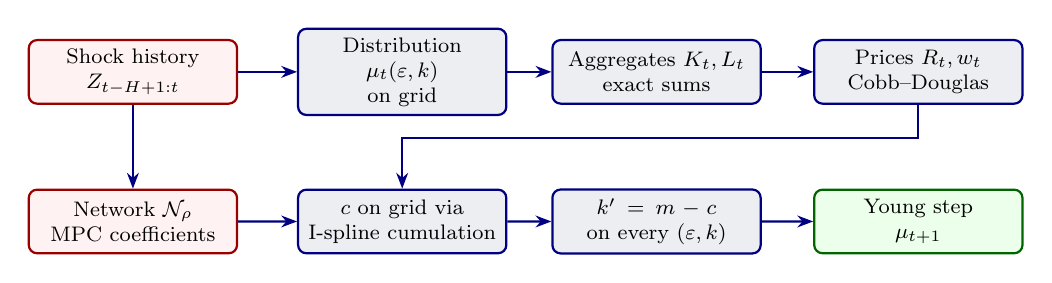
\begin{tikzpicture}[scale=0.95, every node/.style={transform shape},
    box/.style={rectangle, rounded corners=3pt, draw=uzhblue, thick,
        fill=uzhgreylight, text width=2.55cm, minimum height=0.85cm,
        align=center, font=\footnotesize},
    boxr/.style={rectangle, rounded corners=3pt, draw=harvardcrimson, thick,
        fill=red!5, text width=2.55cm, minimum height=0.85cm,
        align=center, font=\footnotesize},
    boxg/.style={rectangle, rounded corners=3pt, draw=darkgreen, thick,
        fill=green!8, text width=2.55cm, minimum height=0.85cm,
        align=center, font=\footnotesize},
    arr/.style={-{Stealth[length=2mm]}, thick, uzhblue}
]
    \node[boxr] (zh) at (0,0) {Shock history\\ $Z_{t-H+1{:}t}$};
    \node[box] (mu)  at (3.6,0) {Distribution $\mu_t(\varepsilon,k)$\\ on grid};
    \node[box] (KL)  at (7.0,0) {Aggregates $K_t,L_t$\\ exact sums};
    \node[box] (P)   at (10.5,0) {Prices $R_t,w_t$\\ Cobb--Douglas};

    \node[boxr] (net) at (0,-2.0) {Network $\mathcal{N}_\rho$\\ MPC coefficients};
    \node[box]  (c)   at (3.6,-2.0) {$c$ on grid via\\ I-spline cumulation};
    \node[box]  (kp)  at (7.0,-2.0) {$k' = m - c$\\ on every $(\varepsilon,k)$};
    \node[boxg] (yo)  at (10.5,-2.0) {Young step\\ $\mu_{t+1}$};

    \draw[arr] (zh) -- (mu); \draw[arr] (mu) -- (KL); \draw[arr] (KL) -- (P);
    \draw[arr] (zh.south) -- (net.north);
    \draw[arr] (P.south) -- ++(0,-0.45) -| (c.north);
    \draw[arr] (net) -- (c); \draw[arr] (c) -- (kp); \draw[arr] (kp) -- (yo);
\end{tikzpicture}

\vspace{0.3em}
\begin{block}{Why Young inside the simulator}
Aggregates $K = \sum k\,\mu(\varepsilon,k)$ and $L = \sum \varepsilon\,\mu$ are \emphc{exact weighted sums} on the grid.  No Monte-Carlo noise floor on prices.
\end{block}
\end{frame}


\begin{frame}{KS Tutorial: Fischer--Burmeister KKT Loss}
\small
\begin{columns}[T]
\column{0.50\textwidth}
\textbf{Two regimes per household}
\begin{itemize}\itemsep2pt
    \item Interior $(k'>0)$: Euler holds with equality, $g=0$.
    \item Constrained $(k'=0)$: Euler gap $g\ge 0$.
\end{itemize}

\textbf{Residuals on the grid}
\[
g \;=\; \frac{c_{\text{Euler}}-c}{c}, \qquad s \;=\; \frac{k'}{c}.
\]
With $c_{\text{Euler}} = 1/q$ and
\[
q \;=\; \beta\,\mathbb{E}_t\!\bigl[\,R'\,u'(c')\bigr]
\]
evaluated by integrating across $(\varepsilon',Z')$.

\column{0.49\textwidth}
\textbf{Fischer--Burmeister envelope}
\[
\mathrm{FB}(g,s) \;=\; \sqrt{g^2 + s^2 + \epsilon_{\text{fb}}} - g - s.
\]
$\mathrm{FB}=0$ iff KKT holds.

\medskip
\begin{block}{Loss}
\[
\mathcal{L}(\rho) \;=\; \mathbb{E}_{\text{buffer}}\Bigl[\overline{\mathrm{FB}^2}\Bigr]
\]
mean over the $(\varepsilon,k)$ grid, averaged over replay states.
\end{block}
\end{columns}
\end{frame}


\begin{frame}{KS Tutorial: Replay Buffer and Training Loop}
\small
\begin{columns}[T]
\column{0.50\textwidth}
\textbf{Buffer state} = pair $(Z\text{-history},\,\mu)$.

\smallskip
\textbf{Each epoch}
\begin{enumerate}\itemsep2pt
    \item Draw $N_{\text{agg}}$ buffer entries; new shock paths.
    \item Roll forward $T$ periods with current $\mathcal{N}_\rho$ to update $\mu$ via Young (\texttt{stop\_gradient}).
    \item Append terminal $(Z\text{-hist},\mu)$ pairs, evict oldest.
    \item Take \texttt{FB\_STEPS} mini-batch SGD steps on $\mathrm{FB}^2$.
\end{enumerate}

\column{0.46\textwidth}
\textbf{Notebook defaults}
\begin{center}\renewcommand{\arraystretch}{0.95}
{\footnotesize
\begin{tabular}{ll}
\toprule
History length $H$ & 50\\
Roll-forward $T$   & 100\\
Buffer cap         & 128\\
$N_{\text{agg}}$ per epoch & 8\\
FB steps per epoch & 10\\
FB mini-batch      & 16\\
Optimiser          & Adam, $5\!\times\!10^{-5}$\\
Grad clip          & $\|\cdot\|_2 \le 1$\\
\bottomrule
\end{tabular}}
\end{center}
\end{columns}
\end{frame}


% --- Alternative algorithm + diagnostics + heuristics ----------------

\begin{frame}{Two Training Algorithms: Residual Min vs.\ Time Iteration}
\small
\begin{columns}[T]
\column{0.50\textwidth}
\textbf{Direct residual minimisation}
\begin{itemize}\itemsep2pt
    \item Train on $\mathbb{E}[\mathrm{FB}^2]$ via SGD.
    \item One loss, one optimiser.
    \item Best for smooth, single-root Euler equations.
\end{itemize}

\column{0.49\textwidth}
\textbf{Time iteration with EGM}\\[2pt]
{\footnotesize\itshape (Carroll, 2006; Azinovic-Yang \& \v{Z}emli\v{c}ka, 2025)}
\begin{itemize}\itemsep2pt
    \item Each outer step: use $\mathcal{N}_\rho$ for next-period policy, EGM-invert to get current targets, regress.
    \item Per-batch root-finding step.
    \item Handles \emphc{non-convex} choices, \emphc{multiple roots}, ZLB, non-monotone Laffer.
\end{itemize}
\end{columns}

\vspace{0.2em}
\begin{block}{When to switch}
{\footnotesize Use \emphc{residual minimisation} by default.  Switch to \emphc{time iteration} when convergence stalls, when the Euler equation has multiple roots, or when discrete choices appear in the optimization.}
\end{block}
\end{frame}


\begin{frame}{KS Tutorial: What the Diagnostics Show}
\small
\begin{columns}[T]
\column{0.49\textwidth}
\textbf{Convergence}
\begin{itemize}\itemsep2pt
    \item $\log \mathrm{FB}^2$ vs.\ epoch.
    \item Target accuracy $\sim\!10^{-6}$ on the simplified KS economy.
\end{itemize}

\textbf{Learned policy}
\begin{itemize}\itemsep2pt
    \item $c(k)$ and MPC plotted at all-low and all-high $Z$ histories.
    \item Differences across $Z$ histories reveal how the network reads aggregate state through the shock window.
\end{itemize}

\column{0.49\textwidth}
\textbf{Approximate aggregation scatter}
\begin{itemize}\itemsep2pt
    \item Plot $c(\varepsilon, k)$ and MPC at fixed $k$ against $K$ across replay states.
    \item Tight clouds = the policy depends mainly on contemporaneous prices.
\end{itemize}

\textbf{Euler/FB error bands}
\begin{itemize}\itemsep2pt
    \item Median and 10--90\% percentile bands of $|\mathrm{FB}|$ across the buffer.
    \item Higher near the constraint $k\!\approx\!0$ and at high $k$ with little household mass.
\end{itemize}
\end{columns}
\end{frame}


\begin{frame}{Practical Heuristics}
\small
\begin{block}{Truncation length $T$ -- three rules}
{\footnotesize
\begin{enumerate}\itemsep1pt
    \item \textbf{OLG:} two life-cycles (covers all shocks experienced by any living household).
    \item \textbf{Iterative:} start short, increase until residual stops dropping.
    \item \textbf{Overkill:} $\rho_{\text{shock}}^T \le 10^{-8}$.  Long histories are cheap to feed.
\end{enumerate}}
\end{block}

\begin{columns}[T]
\column{0.49\textwidth}
\begin{block}{Innovations or realisations?}
{\footnotesize For AR(1) shocks, feed \emphc{realisations} $z_t^T$ rather than innovations $\varepsilon_t^T$.  Levels integrate the persistence, so shorter $T$ suffices.  Feeding both is most accurate.}
\end{block}

\column{0.49\textwidth}
\begin{block}{What to approximate}
{\footnotesize Smooth, bounded objects (\emphc{MPCs, savings rates}) yield much better Euler accuracy than raw levels (consumption, savings).  This is why I-spline MPCs work so well.}
\end{block}
\end{columns}

\begin{alertblock}{When the method breaks}
{\footnotesize Truncation relies on \emph{ergodicity}: $\partial\Psi/\partial\varepsilon_{t-\tau}\to 0$ as $\tau\to\infty$.  Limit cycles or deterministic chaos violate this; convergence is then not guaranteed.}
\end{alertblock}
\end{frame}

\end{document}
